\begin{figure}[htb]
\centering
\includegraphics[width=0.45\textwidth]{\FCNCFigures/tthML/showFake/faketau/prefit/NOMINAL/reg2l1tau1bnj/tau_pt_0.pdf}
\put(-100, 140){\textbf{(a1)}}
\put(-120, 130){\footnotesize{$2l1tau1b$}}
\includegraphics[width=0.45\textwidth]{\FCNCFigures/tthML/showFake/faketau/prefit/NOMINAL/reg2l1tau2bnj/tau_pt_0.pdf}
\put(-100, 140){\textbf{(a2)}}
\put(-120, 130){\footnotesize{$2l1tau2b$}}

\includegraphics[page=6,width=0.45\textwidth]{\FCNCFigures/tthML/showFake/faketau/prefit/NOMINAL/reg1l1tau2b2j_os/tau_pt_0.pdf}
\put(-100, 140){\textbf{(b1)}}
\put(-120, 130){\footnotesize{$1l1tau2b2j OS$}}
\includegraphics[page=6,width=0.45\textwidth]{\FCNCFigures/tthML/showFake/faketau/prefit/NOMINAL/reg1l1tau2b3j_os/tau_pt_0.pdf}
\put(-100, 140){\textbf{(b2)}}
\put(-120, 130){\footnotesize{$1l1tau2b3j OS$}}

\includegraphics[page=6,width=0.45\textwidth]{\FCNCFigures/tthML/showFake/faketau/prefit/NOMINAL/reg1l1tau2b2j_ss/tau_pt_0.pdf}
\put(-100, 140){\textbf{(c1)}}
\put(-120, 130){\footnotesize{$1l1tau2b2j SS$}}
\includegraphics[page=6,width=0.45\textwidth]{\FCNCFigures/tthML/showFake/faketau/prefit/NOMINAL/reg1l1tau2b3j_ss/tau_pt_0.pdf}
\put(-100, 140){\textbf{(c2)}}
\put(-120, 130){\footnotesize{$1l1tau2b3j SS$}}

\caption{ The distributions of $\tau$ $\pt$ in the control regions used to calibrate the fake taus. }
\label{fig:wjet_pt_CR}
\end{figure}
